
\chapter{Introduction}

\section{Overview TSHD}
%\textbf{Omschrijving schip werkwijze + kort vulling hopper}
%\textbf{Van Rhee PhD + lecturenotes Dredging processes}

The Trailing suctions hopper dredger (TSHD) is a ship that is equipped with one or two suction pipes, which are lowered to the seabed during dredging operations. A water-sediment mixture is sucked up to the ship which will be discharged in the cargo hold, also called the hopper of the ship. The hopper is filled, where the sand particles settle and excess water flows overboard. The loading process of a TSHD is shown in figure \ref{fig:loading}\citep{Lecture}.\newline

\begin{figure}[ht!]
    \centering
    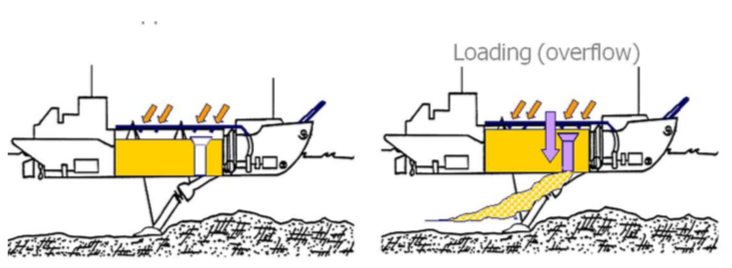
\includegraphics[width=0.8\linewidth]{Images/TSHD_loading.png}
    \caption{Loading process of a TSHD}
    \label{fig:loading}
\end{figure}
\noindent
After the loading process, the TSHD sails to the designated location where the hopper is discharged by opening the doors in the bottom of the ship, pumping the sediment ashore or by rain bowing, which is shown in figure \ref{fig:Rainbow}

\begin{figure}[ht!]
    \centering
    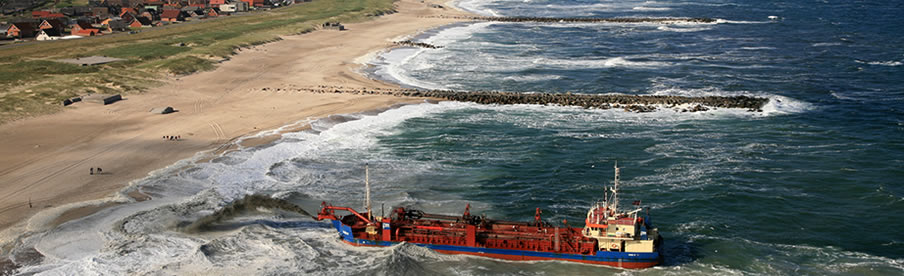
\includegraphics[width=0.8\linewidth]{Images/Rainbow.jpg}
    \caption{Discharge of TSHD by rain bowing}
    \label{fig:Rainbow}
\end{figure}

\noindent
The hopper inlet system varies between ships, but the general aim is to divide the water-sediment mixture over the width of the hopper. During the loading process, the hopper is filled with water to obtain a water level inside the hopper equal to outside. The inlet loading pipes discharge the sucked up water-sediment mixture inside the hopper. The sand particles settle and will form a bed, which grows during the loading process. 




%%%%%%%%%%%%%%%%%%%%%%%%%%%%%%%%%%%%%%%%%%%%%%%%%%%%%%%%%%%%%%%%%%%%%%%%%%%%%%%%%%%%%%%%%%%%%%%%%%%%%%%%%%%%%%%%%%%%%%%%%%%%%%%%%%%%%%%%%%%%%%%%%%%%%%%%%%%%


\section{Description of overflow}

%\textbf{Types of overflow} \newline
%\textbf{Info bij van Rhee winnen} \newline
%\textbf{Tekening overflow (bijlage)}

The excess water flows overboard through the overflow. The commonly used overflows these days are adjustable in the vertical to regulate the overflow in the hopper. An overview of an overflow is shown in figure \ref{fig:Overflow}. 

\begin{figure}[ht!]
    \centering
    \includegraphics[width=0.8\linewidth]{Images/}
    \caption{Cross section of hopper with overflow}
    \label{fig:Overflow}
\end{figure}

\noindent
The overflow will transport the excess water underneath the hull into the surrounding water. However, not every sand particle will settle inside the hopper due to the current from the inlets to the overflow inside the hopper. With the dividing of the water-sediment mixture over the hopper dimension the process is more or less controlled to load as fast as possible, and so, to lose as less sand particles through the overflow. Despite this, the control of the process is very hard and so sand particles are lost through the overflow.\newline

%Werking Overflow vragen Vrhee / Rhode Nielsen




%%%%%%%%%%%%%%%%%%%%%%%%%%%%%%%%%%%%%%%%%%%%%%%%%%%%%%%%%%%%%%%%%%%%%%%%%%%%%%%%%%%%%%%%%%%%%%%%%%%%%%%%%%%%%%%%%%%%%%%%%%%%%%%%%%%%%%%%%%%%%%%%%%%%%%%%%%%%


\section{Ecological effects of sediment turbidity}
The dredging process with a TSHD may lead to increased turbidity, higher suspended concentrations and enhanced sediment deposition. This mainly affects performance of visual predators and growth and survival of bottom vegetation as is shown in figure \ref{fig:Ecoligical}. However it is not understood yet, how large this impact is and whether it results in real problems. The circumstances in the sea and on and in the bed may change, but it is not clear if and how it will affect the flora and fauna in this region. The tolerance levels of different species of plant and animals differ from each other. Therefore some species may profit from increased sedimentation or suspended matter concentrations, whilst others do not survive a slight change in living environment. An important aspect is the kind of material that is released into the water. Clay particles together with organic material can form large coagulates that absorb a lot of light, while the organic material is also a source of food. In contrast a same weight of sand particles absorbs almost no light. \citep{Dankers} \newline
Turbidity at a certain distance from the ship can be reduced, however, turbidity around the ships location can not disappear. Therefore the ecological effect of turbidity is more important for passive plumes that travel far field.

\begin{figure}[ht!]
    \centering
    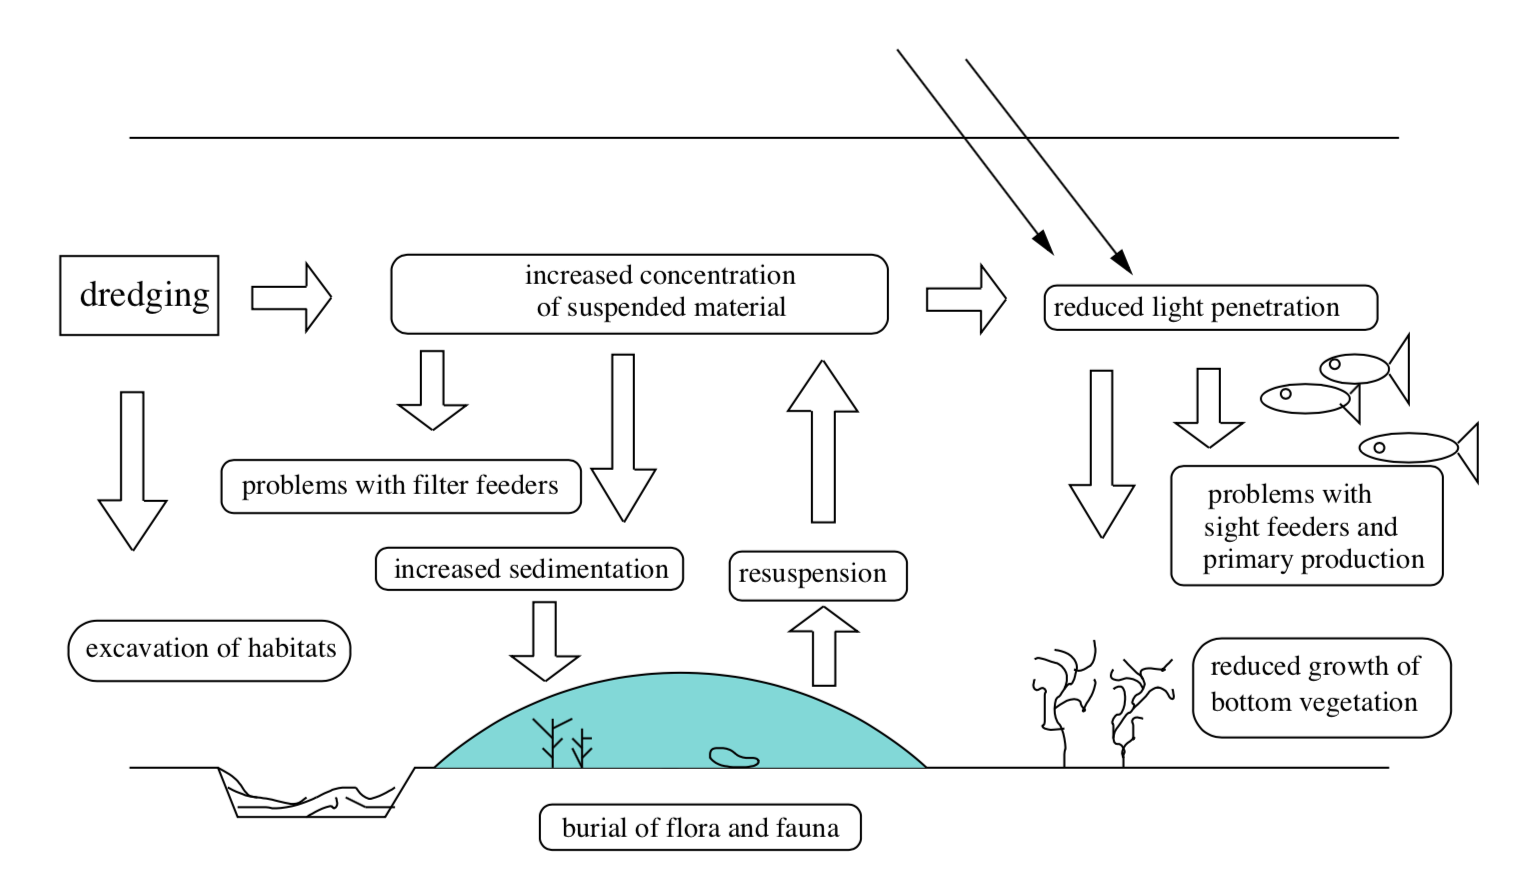
\includegraphics[width=.75\linewidth]{Images/Ecological.png}
    \caption{Ecological effect dredging}
    \label{fig:Ecoligical}
\end{figure}

%%%%%%%%%%%%%%%%%%%%%%%%%%%%%%%%%%%%%%%%%%%%%%%%%%%%%%%%%%%%%%%%%%%%%%%%%%%%%%%%%%%%%%%%%%%%%%%%%%%%%%%%%%%%%%%%%%%%%%%%%%%%%%%%%%%%%%%%%%%%%%%%%%%%%%%%%%%%

\section{Research Aim}

The aim of this master thesis is to provide insight in which factors influence the amount of surface turbidity and provide a practical solution to decrease the surface turbidity. The turbidity has ecological ans visual impact and should be decreased for ecological regulations.

%%%%%%%%%%%%%%%%%%%%%%%%%%%%%%%%%%%%%%%%%%%%%%%%%%%%%%%%%%%%%%%%%%%%%%%%%%%%%%%%%%%%%%%%%%%%%%%%%%%%%%%%%%%%%%%%%%%%%%%%%%%%%%%%%%%%%%%%%%%%%%%%%%%%%%%%%%%%

\section{Research Methodology}

\noindent The research methodology is characterized by the following steps:
\begin{itemize}
    \item Description dredging processes in the near field
    \item Find out which factors influence the creating of a surface plume
    \item Experiments (Practical)
    %\item Practical solution
\end{itemize}  






%%%%%%%%%%%%%%%%%%%%%%%%%%%%%%%%%%%%%%%%%%%%%%%%%%%%%%%%%%%%%%%%%%%%%%%%%%%%%%%%%%%%%%%%%%%%%%%%%%%%%%%%%%%%%%%%%%%%%%%%%%%%%%%%%%%%%%%%%%%%%%%%%%%%%%%%%%%%

\section{Outline}



%%%%%%%%%%%%%%%%%%%%%%%%%%%%%%%%%%%%%%%%%%%%%%%%%%%%%%%%%%%%%%%%%%%%%%%%%%%%%%%%%%%%%%%%%%%%%%%%%%%%%%%%%%%%%%%%%%%%%%%%%%%%%%%%%%%%%%%%%%%%%%%%%%%%%%%%%%%%

%NOMENCLATURE

\nomenclature[Z]{TSHD}{Trailing Suction Hopper Dredger}
\nomenclature[A]{$g$}{Gravity acceleration \nomunit{[$m/s^2$]}}

